\documentclass[report,twocolumn]{aa}
\usepackage{fixltx2e}
\usepackage[english]{babel}
\usepackage{graphicx,amsmath}
%\usepackage{epstopdf}
\usepackage{epsf,color}
\usepackage[mathscr]{eucal}
\usepackage{amsmath}
\usepackage{amssymb,amsfonts}
\usepackage{natbib}
\usepackage{txfonts}
\usepackage{dsfont}
\definecolor{Mygreen}{rgb}{0.00, 0.72, 0.0}
\definecolor{Mypink}{rgb}{1.0, 0.0, 0.5}
\usepackage[breaklinks, citecolor=blue, linkcolor=Mygreen, urlcolor=Mypink, colorlinks=true, debug, baseurl=' ']{hyperref}
\usepackage{float}
\usepackage{color}
%\usepackage{scrextend}
%\usepackage{nccmath}
%\usepackage{mathtools, cuted}
%\usepackage{lscape}
\usepackage{widetext}
%\usepackage{flushend}
%\usepackage[T1]{fontenc}


\newcommand{\nika}{{\it NIKA}}
\newcommand{\nikad}{{\it NIKA2}}


\def\intk#1{\displaystyle\int\frac{d^2k_{#1}}{(2\pi)^2}}
\def\intr#1{\displaystyle\int d^2r_{#1}}
\def\simlt{\lower.5ex\hbox{$\; \buildrel < \over \sim \;$}}
\def\simgt{\lower.5ex\hbox{$\; \buildrel > \over \sim \;$}}
\def\simgt{\lower.5ex\hbox{$\; \buildrel $\textgreater$ \over \sim \;$}}
\def\NIKA{\textit{NIKA}}
\def\NIKAd{\textit{NIKA2}}
\def\Archeops{\textit{Archeops}}
\def\Planck{\textit{Planck}}
\def\WMAP{\textit{WMAP}}
\def\Skydip{\textit{Skydip}}

\bibpunct{(}{)}{;}{a}{}{,}
\bibliographystyle{aa}

\begin{document}
\title{Crab nebula polarization observations at 150 GHz with NIKA: \\ implications for future CMB experiments: Answer to the referee}

\section{First question}

The handling of noise bias, and more generally the discussion of
errors and uncertainties, is not sufficiently sophisticated to meet the
stated goals of this paper (namely that the measurements might be used
for calibration of other instruments). There are two places where
this is most apparent:
\\ \\
In section 3, an effort is made to make statements about the spatially
integrated flux, polarized flux, and polarization angle of the nebula.
This information is potentially valuable for calibration of CMB
instruments, with larger beams. Ultimately the authors settle on a
method where pixels are excluded from the average if the polarized
flux in the pixel is below 3 times the noise level. This is
problematic for several reasons:\\
(a) Because the polarized intensity is distributed differently than
the unpolarized intensity, cutting on polarized brightness will bias
the measurement towards parts of the nebula with a pixels with a
higher polarization degree (p). This will inflate the "average" p
relative to what an experiment with a larger beam would be able to
observe.\\
(b) The reason given for the exclusion is to avoid "noise bias". The
noise bias is described earlier in the paper and is indeed important
when converting low S/N measurements of I,Q,U into estimates of p and
polarization angle (psi). But to compute integrated p and psi values
correctly, one should first obtain integrated values of I, Q, and U;
these will have quite high S/N, compared to individual pixel S/N, and
noise bias will not be a concern.\\
(c) This exclusion is hardly a minor technical point, since it changes
the inferred polarization angle by 3.5 degrees and the polarization
fraction by more than 1 percentage point. For the polarization angle,
at least, this change is much larger than the total uncertainty.
Although the authors perform this computation both with and without
the exclusion of S/N \textless 3 points, the values they carry forward, and
use in summary sentences and plots, are the biased ones (using S/N \textgreater 3
only). One suspects that the S/N \textgreater 3 results were ultimately chosen
because they agree better with the results from other experiments
(WMAP and Planck). The authors mention the need for an "additional
uncertainty at a level of 1\% on p and 4 deg on psi", but this
uncertainty is not mentioned again; it is not included in tables,
plots, or summary sentences.
\\ \\
Secondly, the authors often quote numbers with very small statistical
errors. For example, for one of the averages in section 3, the mean
polarization angle has an error of 0.0004 degrees. This suggests
either a numerical mistake, or that the map noise has been
treated as white when in fact it has significant correlated structure
on angular scales larger than the pixel. In the latter case, a
profitable approach is to check for consistency between different
subsets of the data (e.g., look at two co-adds of 12 maps instead of
the one co-add of 24 maps).

\subsection{\textbf{Answer}}

\section{Second question}
2. Basic errors in astrometry and coordinate handling.
\\
The position of the Crab Pulsar is given, to sufficient precision, in
both the Introduction and the Conclusion. But the position of the
pulsar is not plotted correctly in any of the images that purport to
do so. Rather, the position appears to have been truncated to 0.01
degrees prior to plotting.
\\
The position angle (PA) conversion between galactic and equatorial
coordinates is not done correctly. In tables 1 and 2 we find that the
Equatorial and Galactic PA differ by values ranging between 220 to 245
degrees, even though all of these points lie in a very small region of
the sky.
\\
These issues undermine a reader's confidence that the authors have
performed the photometry as described, or that they understand the
tools used to convert between coordinate systems to a sufficient
degree that we can trust their results.
\subsection{\textbf{Answer}}
\textbf{The error in the pulsar position concerns only the plot.
Indeed we used previous observations from XPOL experiment (Aumont et al. 2010) to match the map and the position of the pulsar.
There was unfortunately a pointing offset between the two instrument (Xpol and NIKA) ``center of the map" for this observation that we have now corrected on maps, see Fig.~\ref{Q_map}.}

{\color{blue}I do not understand the second point of the question, and even if we have decided to compute the polar angles in galactic coordinates for all the experiments, I do not see his point. Moreover to properly calculate the angles I need to know at least the intensity flux, e.g. at the pulsar position. With only p and $\psi$ in Radec coordinates I do not see how to obtain q and u in galactic coordinates and then $\psi_{gal}$.}

\begin{figure}[!h]
\centering
     	  { 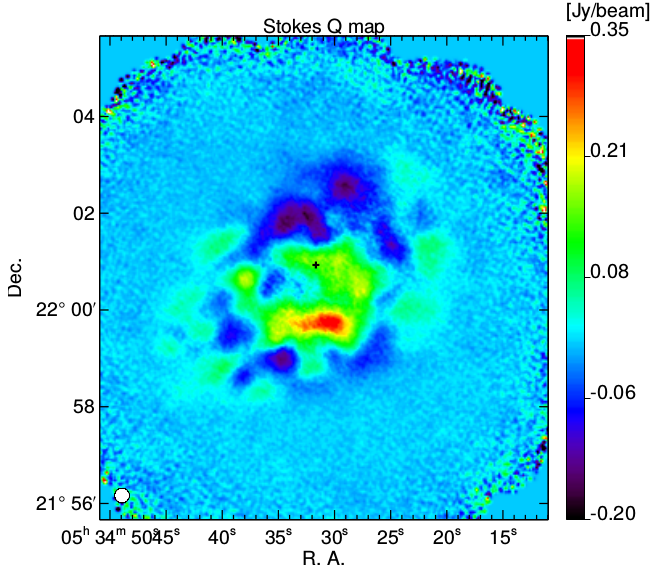
\includegraphics[width=1\linewidth,keepaspectratio]{referee_figures/crab_q_2mm_pulsPositionCor.png}}
\caption{Stokes Q map with pulsar position corrected.}     	  
 
\label{Q_map}
\end{figure}




\section{Third question}
Models are not explained clearly, and fits contain obvious errors.\\
(a) The intensity model described in equations (6) and (7) is not
completely described. It appears to be discontinuous, through 100
GHz, and the best-fit values are only given for 2 of the 4 model
parameters. Fig. 6 shows a very reasonable broken power-law fit to
the data, but the description in the text is inadequate and confusing.\\
(b) In 4.2, models are fit to the polarized intensity from WMAP and
Planck. It is alleged that only data below 100 GHz are used; this
raises the question of whether or not the Planck measurement at 100
GHz is included. The best-fit parameters for Planck, stated in
equation (9) and plotted in Fig. 7, do not appear to be the best fit
to these data. Indeed, if I take the Planck measurements and fit a
simple power-law, I find a very different best-fit line: A = 91.8 and
beta = -0.38.
These errors and/or omissions make it difficult to take any of the
model fitting seriously; they undermine the conclusions of the paper.
\\ \\
\subsection{\textbf{Answer}}
\textbf{(a)  The fit in Fig. 6 appears to be discontinuos because it is due to the sum of two different fits. When we DO NOT consider the Planck data for $\nu$ \textgreater 100 GHz the parameters of the fit are: A = 980.6 +- 0.7 and $\beta$ = -0.3151+-0.0002.
Otherwise, fitting Planck data with $\nu$ \textgreater 100 GHz gives: A$_H$ = 8.6+-0.45 and $\beta$ = -0.71+-0.09.}

{\color{blue} If now we consider to fit all data we obtain the plot of Fig.\ref{crab_int_SED}
where the cut-off frequency is 90 GHz and the knee frequencies are: 8 GHz and 100 GHz. See the code fading-2sync.pro in my labtool under the subdirectories codes4thesis and CRAB.
The best-fit parameters using the code plot-SED-intensity.pro are:
} 
 \begin{equation}
 A_1 = 507.7+-0.1 \quad \beta_1 = -0.31866+-5x10^{-5} \nonumber
 \end{equation}
 and
 \begin{equation}
 A_2 = 216.36+-0.33 \quad \beta_2 = -0.7525+-0.0003
 \end{equation}



\begin{figure}[!ht]
\centering
     	  { 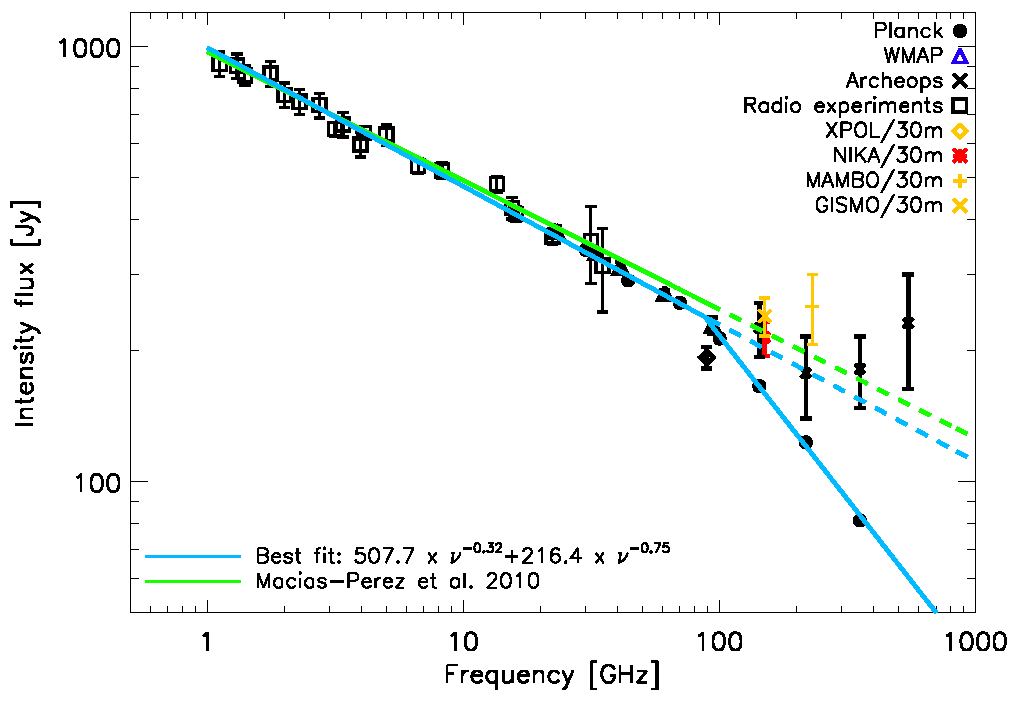
\includegraphics[width=1\linewidth,keepaspectratio]{referee_figures/Crab_SED_int_test.pdf}}
\caption{Total intensity SED.}     	  
 
\label{crab_int_SED}
\end{figure}


\textbf{(b) The models represented in Fig.7 account for the data at frequecies below 100 GHz. If we take now into account all data we obtain:
A = 116.5+-6.52 for the amplitude and $\beta$ = -0.45+0.01.
And, considering an uncertainty of 0.1 fixed for all data we obtain:
A = 89.85+-1.22 and $\beta$ = -0.389+-0.003; see Fig.~\ref{crab_polar_SED}}
\begin{figure*}[h!]
  \centering
     	  { 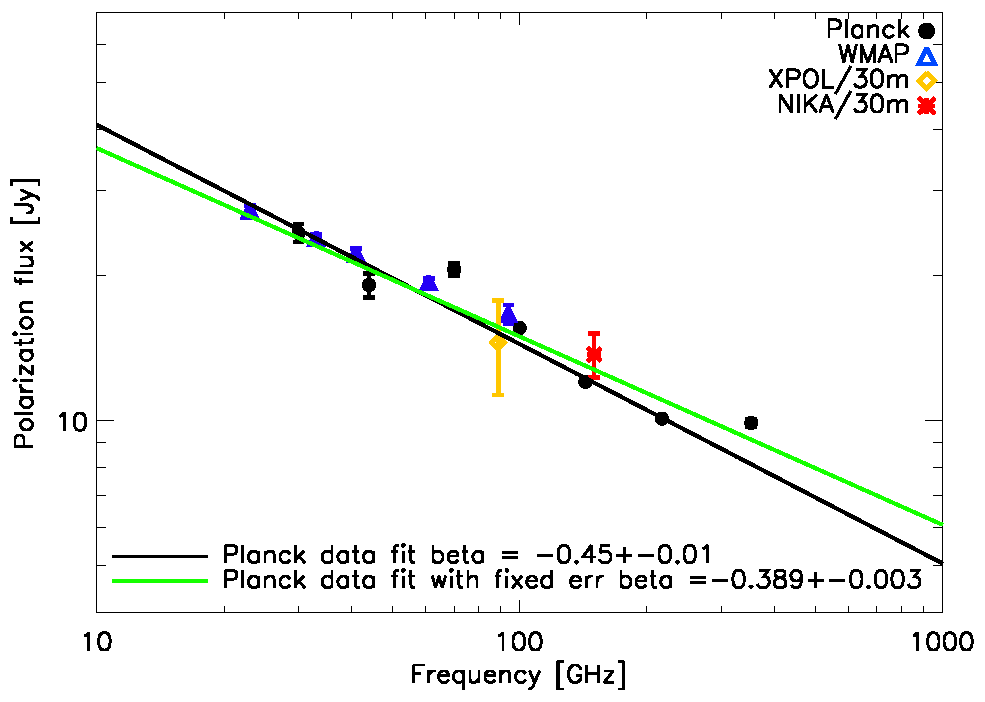
\includegraphics[width=0.5\linewidth,keepaspectratio]{referee_figures/Crab_SED_ipol_test.pdf}}
     	  \caption{Polarization SED.}  
     	\label{crab_polar_SED}
\end{figure*}
  



\end{document}
